\subsubsection{Schaltungsaufbau} \label{subsec:schaltungsaufbau}

Das vorgegebene EMI-Filter muss bezüglich der Einfügungsverluste (Insertion Loss) untersucht werden. Die Einfügunsverluste hängen vom Gesamtrauschen der Schaltung ab. Es wird ein Ansatz verwendet, der in der Praxis weit verbreitet ist, bei welchem das Gesamtrauschen in zwei Komponenten unterteilt wird. Man spricht vom Gegen-(=Differential Mode=DM) und Gleichtaktrauschen (=Common Mode=CM). Anhand der vorgegebenen CM- und DM-Äquivalenten Schaltungen (Abbildungen \ref{fig:CM-Schaltungäquivalent}, \ref{fig:DM-Schaltungsäquivalent})werden die Einfügungsverluste in Funktion der Frequenz berechnet. Die Berechnungen decken einen Bereich von 0 bis 30MHz ab. 


 
\newpage

Die Schaltung \ref{fig:orig_Schaltung} \nameref{fig:orig_Schaltung} zeigt den Filteraufbau, wie er der Aufgabenstellung zu entnehmen ist. Um das Gegentaktrauschen und das Gleichtaktrauschen bestimmen zu können, werden die beiden Schaltungsäquivalente gebildet. 
\begin{figure}[H]
	\centering
	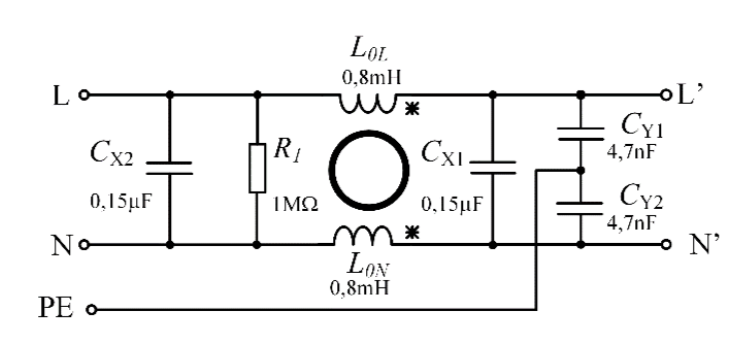
\includegraphics[width = 10cm]{orig_ElectricalCircuit.png}
	\caption{Original Schaltung \cite{aufgabenstellung}}
	\label{fig:orig_Schaltung}
\end{figure}


%TODO Die Schaltungsäquivalenzen müssen aufgeteilt werden und in die jeweiligen subsubsections gekippt werden
